\part{Seriel/Parallel Kommunikation}
\chapter{Grundlæggende Seriel og Parallel Kommunikation}
\section{Introduktion til Seriel Kommunikation}
Seriel kommunikation er en metode til at overføre data, hvor bits sendes én efter én over en enkelt kommunikationskanal eller tråd. Dette står i kontrast til parallel kommunikation, hvor flere bits sendes samtidigt over flere tråde. Seriel kommunikation er almindeligt anvendt i forskellige industrielle applikationer på grund af dens enkelhed og effektivitet, især over lange afstande.
\newline\newline\noindent
I industrielle systemer bruges seriel kommunikation ofte til at forbinde enheder som PLC'er, sensorer, og aktuatorer, der kræver en pålidelig og relativt langsom dataoverførsel. De mest anvendte serielle kommunikationsstandarder inkluderer RS232, RS422, og RS485, som alle har forskellige fordele afhængigt af applikationen og miljøet.
\newline\newline\noindent
Seriel kommunikation er populær i industrielle miljøer på grund af dens evne til at operere over lange kabellængder med lav støjfølsomhed. Sammenlignet med parallel kommunikation kræver seriel kommunikation færre forbindelser, hvilket reducerer kompleksiteten og omkostningerne ved installation og vedligeholdelse.
\newline\newline\noindent
I dette afsnit vil vi udforske grundlæggende begreber inden for seriel kommunikation, herunder de mest anvendte standarder og deres specifikationer. Vi vil også se på praktiske anvendelser af seriel kommunikation i industrielle netværk samt de udfordringer og løsninger, der er forbundet med denne kommunikationsform.

\section{Bits, Bytes og Tegn}
En computer anvender det binære talsystem, som kun har to cifre, 0 og 1. Ethvert tal kan repræsenteres ved en streng af disse cifre, kendt som bits (fra binært ciffer). For eksempel svarer det decimale tal 5 til det binære tal 101.
\begin{table}[h]
	\centering
	\begin{tabular}{|l|l|}
		\hline
		Bit & 1 eller 0 \\ \hline
		Dibit & To bits (10) \\ \hline
		Nibble & Fire bits (1001 eller et Hex-tegn) \\ \hline
		Byte & Otte bits eller to nibbles (11000001, C1 Hex) \\ \hline
		Word & Bredden af computerens bus \\ \hline
	\end{tabular}
	\caption{Forskellige sæt af bits}
	\label{tab:bits_sets}
\end{table}
Da en bit kun kan have to værdier, kan den repræsenteres af en spænding, der enten er tændt (1) eller slukket (0). Dette kaldes også logisk 1 og logisk 0. Typiske værdier, der bruges i en computer, er 0 V for logisk 0 og +5 V for logisk 1, selvom det også kan være omvendt, dvs. 0 V for 1 og +5 V for 0.
\newline\newline\noindent 
En streng af otte bits kaldes en 'byte' (eller oktet) og kan have værdier, der spænder fra 0 (0000 0000) til 255\(_{10}\) (1111 1111\(_{2}\)). Computere manipulerer generelt data i bytes eller multipla af bytes.
\begin{table}[h]
	\centering
	\begin{tabular}{|c|c|c|}
		\hline
		Decimal & Hexadecimal & Binær \\ \hline
		0 & 0 & 0000 \\ \hline
		1 & 1 & 0001 \\ \hline
		2 & 2 & 0010 \\ \hline
		3 & 3 & 0011 \\ \hline
		4 & 4 & 0100 \\ \hline
		5 & 5 & 0101 \\ \hline
		6 & 6 & 0110 \\ \hline
		7 & 7 & 0111 \\ \hline
		8 & 8 & 1000 \\ \hline
		9 & 9 & 1001 \\ \hline
		10 & A & 1010 \\ \hline
		11 & B & 1011 \\ \hline
		12 & C & 1100 \\ \hline
		13 & D & 1101 \\ \hline
		14 & E & 1110 \\ \hline
		15 & F & 1111 \\ \hline
	\end{tabular}
	\caption{Den hexadecimale tabel}
	\label{tab:hex_table}
\end{table}
Programmører bruger 'hexadecimal' notation, fordi det er en mere bekvem måde at definere og håndtere bytes på. I det hexadecimale talsystem er der 16 cifre (0–9 og A–F), som hver repræsenteres af fire bits. En byte repræsenteres derfor af to hexadecimale cifre.
\newline\newline\noindent 
Et 'tegn' er et symbol, der kan udskrives. Alfabetet, både store og små bogstaver, tal, tegnsætningstegn og symboler som '*' og '\&' er alle tegn. En computer skal kunne udtrykke disse tegn på en sådan måde, at de kan forstås af andre computere og enheder. Den mest almindelige kode til at opnå dette er den amerikanske standardkode for informationsudveksling (ASCII) beskrevet i afsnit 2.8.

\section{Kommunikationsprincipper}
Ethvert datakommunikationssystem kræver følgende komponenter:
\begin{itemize}
	\item En datakilde (en sender eller linjedriver), som konverterer informationen til en form, der er egnet til transmission over en forbindelse.
	\item En modtager, der modtager signalet og konverterer det tilbage til de oprindelige data.
	\item En kommunikationsforbindelse, der transporterer signalerne. Dette kan være kobberledninger, optiske fibre, og radio- eller satellitforbindelser.
\end{itemize}
Derudover skal senderen og modtageren kunne forstå hinanden. Dette kræver enighed om en række faktorer. De vigtigste er:
\begin{itemize}
	\item Den anvendte signaleringstype.
	\item Definitionen af en logisk '1' og en logisk '0'.
	\item De koder, der repræsenterer symbolerne.
	\item Opretholdelse af synkronisering mellem sender og modtager.
	\item Hvordan dataflowet kontrolleres, så modtageren ikke bliver overbelastet.
	\item Hvordan man opdager og korrigerer transmissionsfejl.
\end{itemize}
De fysiske faktorer kaldes 'grænsefladestandard'; de andre faktorer udgør 'protokoller'.
\newline\newline\noindent 
Den fysiske metode til at overføre data over en kommunikationsforbindelse varierer afhængigt af det anvendte medium. For eksempel kan de binære værdier 0 og 1 signaleres ved tilstedeværelsen eller fraværet af en spænding på en kobberledning, ved et par af lydtoner genereret og dekodet af et modem i tilfælde af telefonisystemet, eller ved brug af moduleret lys i tilfælde af optisk fiber.

\section{Kommunikationsmodi}
I ethvert kommunikationslink, der forbinder to enheder, kan data sendes i en af tre kommunikationsmodi. Disse er:
\begin{itemize}
	\item Simplex
	\item Half duplex
	\item Full duplex
\end{itemize}
En simplex system er designet til at sende beskeder i én retning. Dette er illustreret i Figur \ref{fig:simplex}.
\begin{figure}[h]
	\centering
	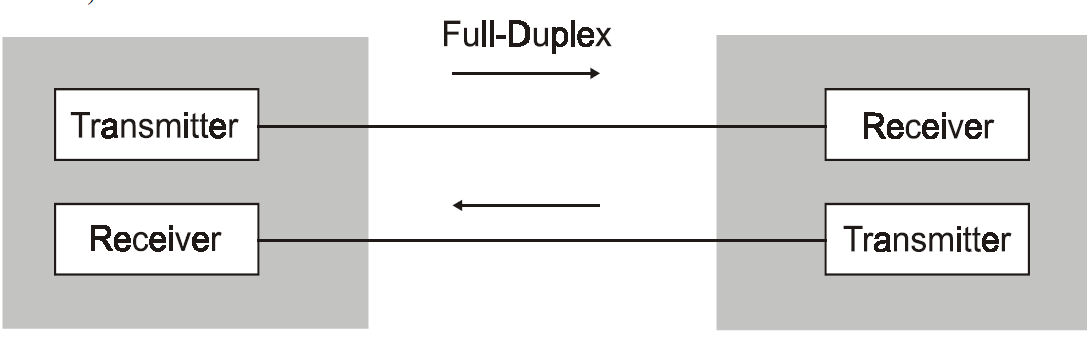
\includegraphics[width=0.6\textwidth]{fig/fig18.png}
	\caption{Simplex kommunikation}
	\label{fig:simplex}
\end{figure}

\noindent Et duplex system er designet til at sende beskeder i begge retninger. Half duplex opstår, når data kan strømme i begge retninger, men kun i én retning ad gangen (Figur \ref{fig:half-duplex}).
\begin{figure}[h]
	\centering
	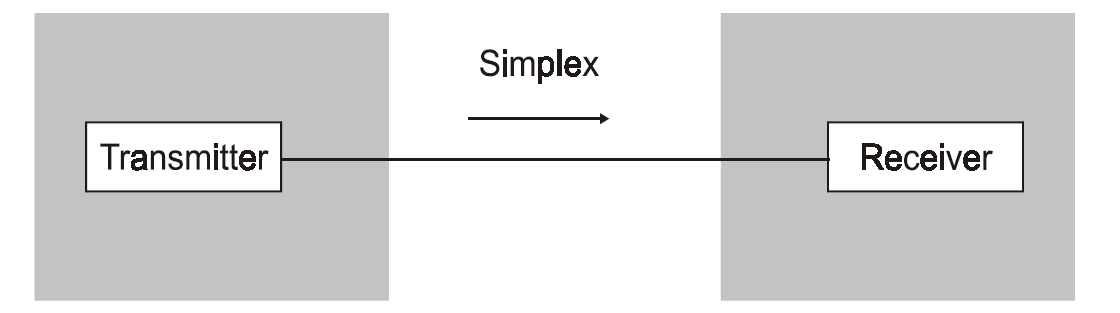
\includegraphics[width=0.6\textwidth]{fig/fig19.png}
	\caption{Half-Duplex kommunikation}
	\label{fig:half-duplex}
\end{figure}

\noindent I et full-duplex system kan data strømme i begge retninger samtidig (Figur \ref{fig:full-duplex}).
\begin{figure}[h]
	\centering
	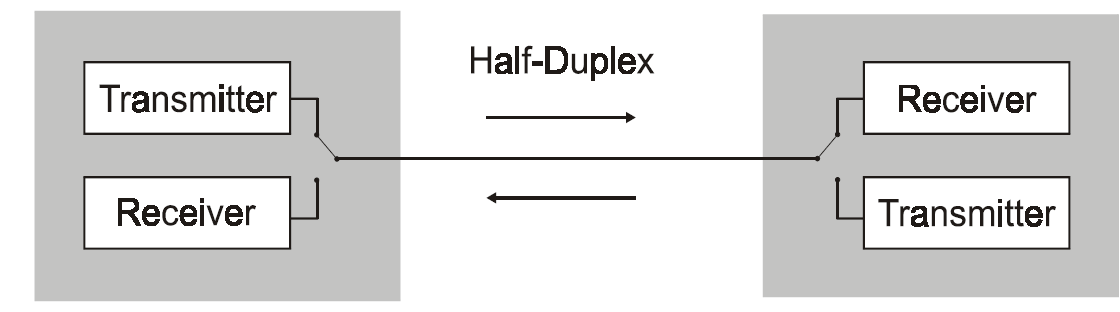
\includegraphics[width=0.6\textwidth]{fig/fig20.png}
	\caption{Full-Duplex kommunikation}
	\label{fig:full-duplex}
\end{figure}

\section{Asynkrone systemer}
Et asynkront system er et, hvor hvert tegn eller byte sendes inden for en ramme. Modtageren begynder ikke at detektere, før den modtager den første bit, kendt som 'startbiten'.
\newline\newline\noindent
\textbf{Startbit:} Startbiten er i den modsatte spændingstilstand i forhold til hvilspændingen og tillader modtageren at synkronisere med senderen for de følgende data i rammen.
\newline\newline\noindent
\textbf{Modtagelse af bits:} Modtageren læser de enkelte bits i rammen, efterhånden som de ankommer, og ser enten logisk 0-spændingen eller logisk 1-spændingen på det rette tidspunkt. 'Clock'-hastigheden i hver ende skal være den samme, så modtageren ser efter hver bit på det tidspunkt, hvor senderen sender den.
\newline\newline\noindent
\textbf{Synkronisering:} Da urene er synkroniseret i starten af hver ramme, kan der tolereres nogen variation ved lavere transmissionshastigheder. Den tilladte variation falder, når dataoverførselshastighederne stiger, og asynkron kommunikation kan have problemer ved høje hastigheder (over 100 kbps).

\section{Meddelelsesformat}
En asynkron ramme kan have følgende format:
\begin{itemize}
	\item \textbf{Startbit:} Signalerer starten af rammen
	\item \textbf{Data:} Normalt 7 eller 8 bits data, men kan være 5 eller 6 bits
	\item \textbf{Paritetsbit:} Valgfri fejldetektionsbit
	\item \textbf{Stopbit(er):} Normalt 1, 1,5 eller 2 bits. En værdi på 1,5 betyder, at niveauet holdes 1,5 gange så længe som en enkelt bit.
\end{itemize}

\begin{figure}[h]
	\centering
	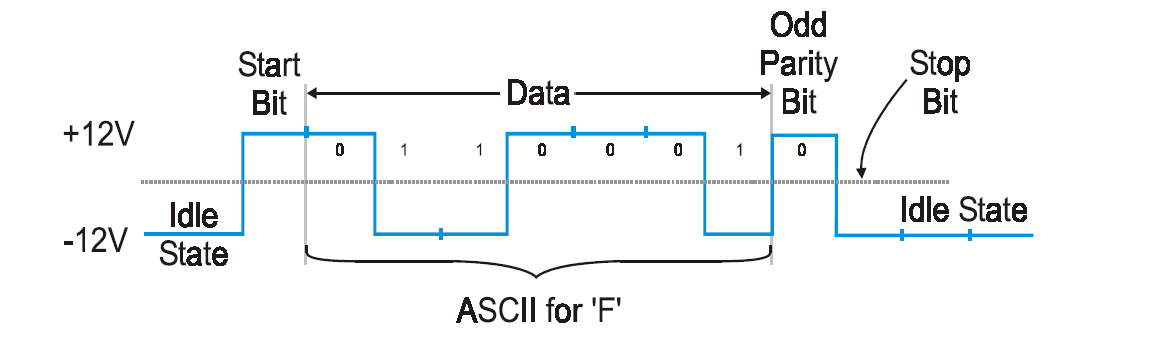
\includegraphics[width=0.8\textwidth]{fig/fig21.png}
	\caption{Asynkront rammeformat}
	\label{fig:asynchronous_frame}
\end{figure}
\noindent Et asynkront rammeformat er vist i Figur \ref{fig:asynchronous_frame}. Senderen og modtageren skal indstilles til præcis den samme konfiguration, så dataene kan udtrækkes korrekt fra rammen. Da hvert tegn har sin egen ramme, er den faktiske dataoverførselshastighed mindre end bithastigheden. For eksempel, med en startbit, syv databits, en paritetsbit og en stopbit, er der ti bits nødvendige for at sende syv bits data. Derfor er transmissionen af nyttige data 70\% af den samlede bithastighed.

\section{Synkrone systemer}
I synkrone systemer synkroniserer modtageren indledningsvis til senderens klokkeimpulser, som er indlejret i de transmitterede datastrømme. Dette gør det muligt for modtageren at opretholde sin synkronisering gennem store beskeder, som typisk kan være op til 4500 bytes (36 000 bits). Dette tillader store rammer at blive transmitteret effektivt ved høje datahastigheder. Det synkrone system pakker mange tegn sammen og sender dem som en kontinuerlig strøm, kaldet en pakke eller en ramme.

\section{Meddelelsesformat}
Et typisk synkront system rammeformat er vist i Figur \ref{fig:synchronous_frame}.
\begin{figure}[h]
	\centering
	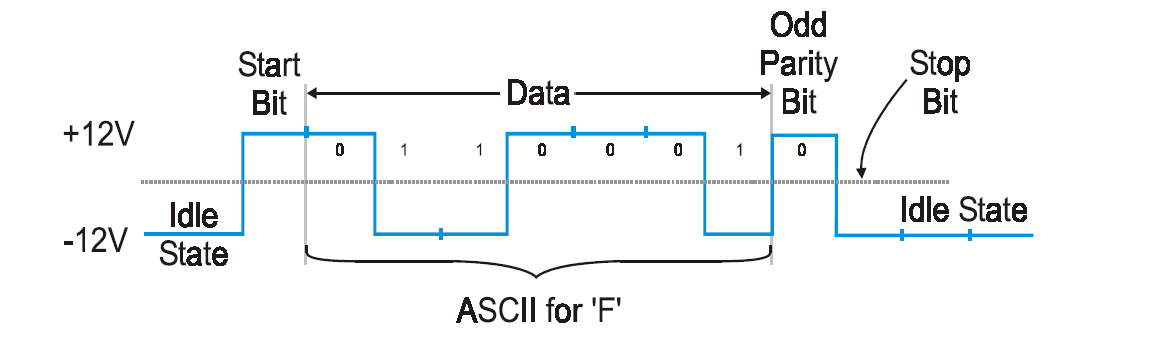
\includegraphics[width=0.8\textwidth]{fig/fig21.png}
	\caption{Typisk synkront system rammeformat}
	\label{fig:synchronous_frame}
\end{figure}

\begin{itemize}
	\item \textbf{Preamble:} Dette omfatter en eller flere bytes, der gør det muligt for modtageren at synkronisere med rammen.
	\item \textbf{SFD:} Start af ramme delimitter signalerer starten af rammen.
	\item \textbf{Destination:} Adressen, som rammen sendes til.
	\item \textbf{Source:} Adressen, som rammen stammer fra.
	\item \textbf{Length:} Antallet af bytes i datafeltet.
	\item \textbf{Data:} Den faktiske besked.
	\item \textbf{FCS:} Frame check sequence er til fejldetektion.
\end{itemize}

\paragraph{Definition og Grundlæggende Koncept}
Seriel kommunikation er en teknik, hvor data overføres én bit ad gangen over en enkelt kommunikationskanal, som typisk er en ledning eller et kabel. Denne form for kommunikation bruges ofte, når data skal sendes over længere afstande, eller hvor det er vigtigt at minimere antallet af ledninger, der er nødvendige for kommunikationen.
\newline\newline\noindent
I modsætning til seriel kommunikation involverer parallel kommunikation overførsel af flere bits samtidigt over flere kanaler eller ledninger. Selvom parallel kommunikation kan opnå højere datahastigheder på korte afstande, kræver den flere ledninger og kan være mere udsat for interferens og synkroniseringsproblemer, især over lange afstande.
\newline\newline\noindent
Den primære fordel ved seriel kommunikation er dens enkelhed og pålidelighed, især i miljøer, hvor der er behov for kommunikation over lange kabler. Det reducerede antal ledninger mindsker risikoen for støj og signalforvrængning, hvilket gør seriel kommunikation ideel til mange industrielle applikationer, hvor robusthed og stabilitet er afgørende.
\newline\newline\noindent
Seriel kommunikation anvender typisk standarder som RS232, RS422 og RS485, der hver især har deres egne specifikationer og anvendelsesområder, afhængigt af kravene til datahastighed, rækkevidde og interferensbeskyttelse.

\chapter{Industriel Seriel Kommunikation og Feltbusprotokoller}
\section{RS232}
RS232 (Recommended Standard 232) er en standard for seriel kommunikation, der er udviklet af Electronic Industries Alliance (EIA). Den bruges primært til at forbinde dataterminaludstyr (DTE) såsom computere til datakommunikationsudstyr (DCE) såsom modemmer. RS232-standardens primære formål er at definere elektriske egenskaber, signalering og timing for serielle dataoverførsler mellem enheder.

\subsection{Fysiske Lag}
RS232 definerer det fysiske lag af kommunikationsforbindelsen, herunder stiktyper, kabler og elektriske signaler. Den mest almindelige stiktype er DB9 (9-pins) eller DB25 (25-pins), selvom andre konfigurationer også findes.
\begin{figure}[h]
	\centering
	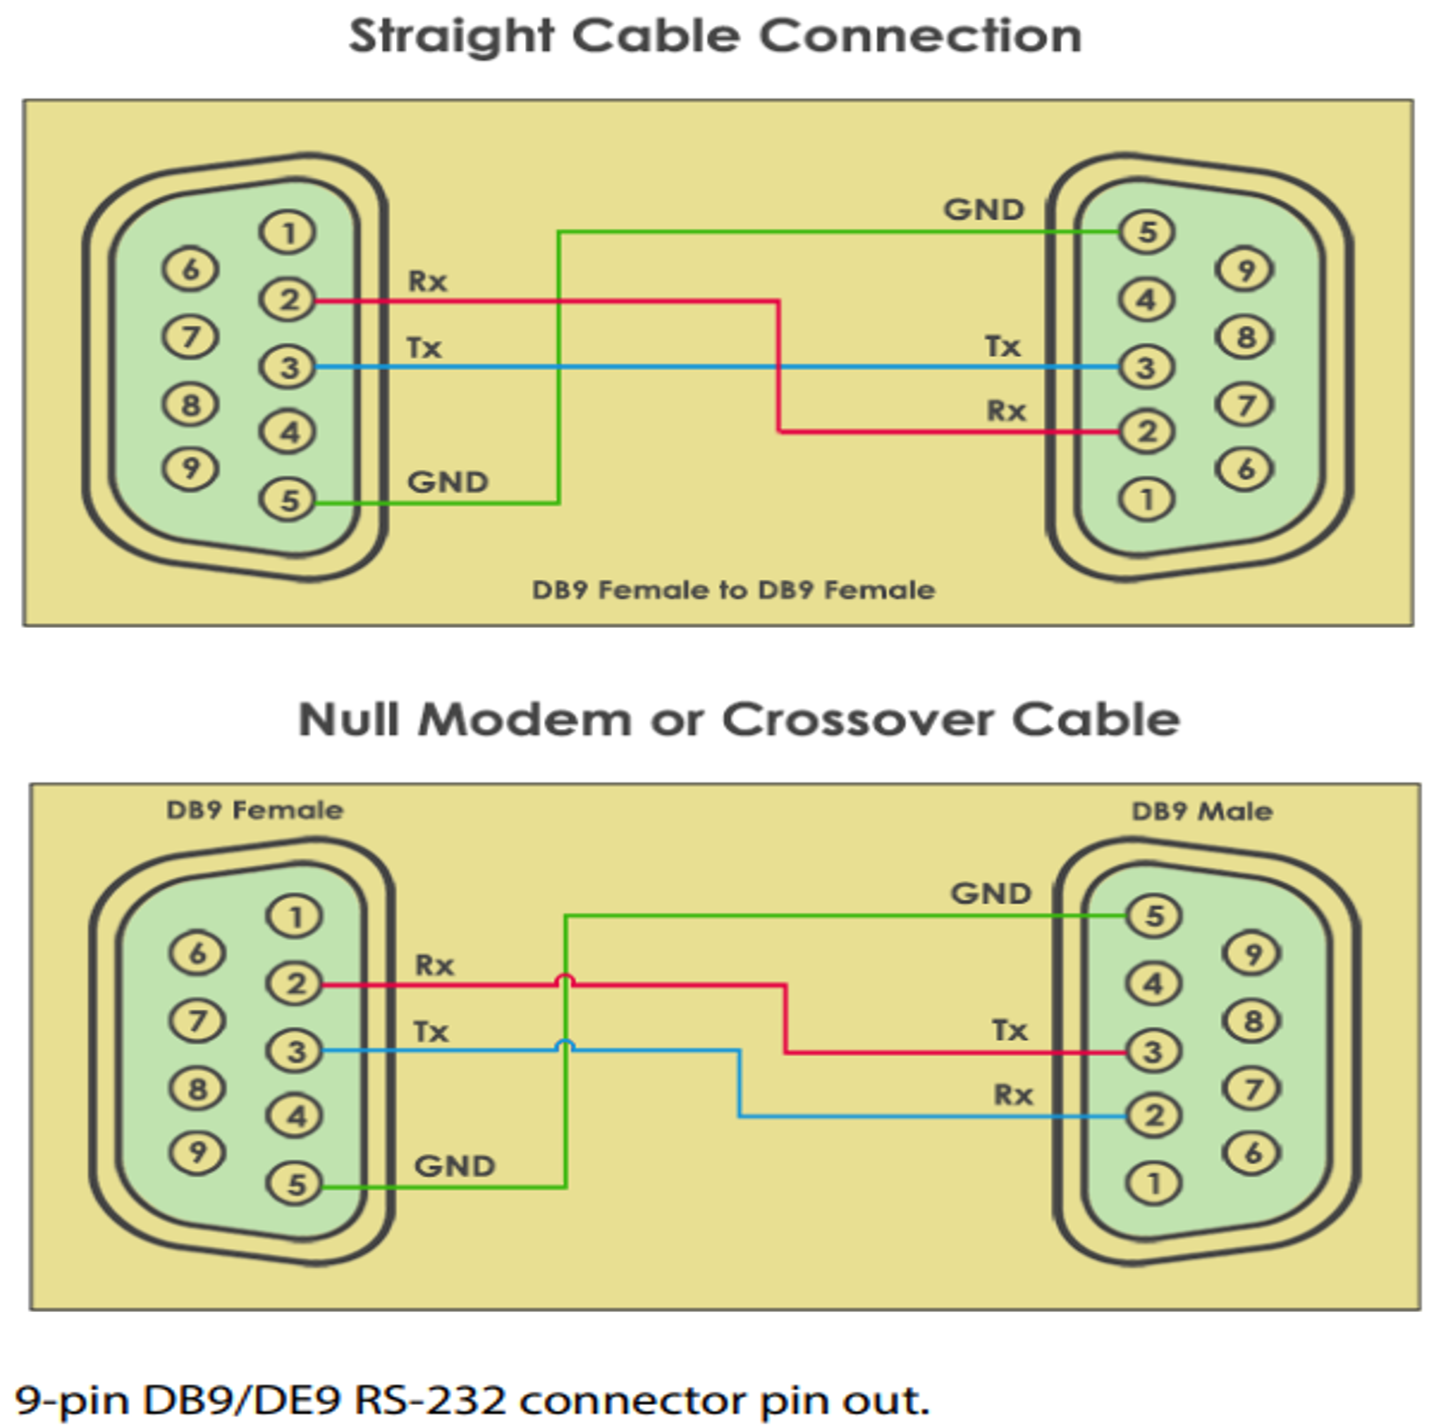
\includegraphics[width=0.5\textwidth]{fig/fig2.png} % Inkluder et billede af RS232-stikket her
	\caption{DB9 stik for RS232}
	\label{fig:rs232_connector}
\end{figure}

\subsection{Elektriske Signaler}
RS232 bruger single-ended signalering, hvilket betyder, at signalet sendes som en spændingsforskel mellem en signalleder og en fælles jordleder. Typiske spændingsniveauer er:

\begin{itemize}
	\item \textbf{Logisk 0 (Marking)}: +3V til +15V
	\item \textbf{Logisk 1 (Spacing)}: -3V til -15V
\end{itemize}
Støjniveauer under ±3V betragtes som udefinerede, hvilket skaber en bufferzone for at minimere signalforstyrrelser.

\subsection{Signalering og Pins}
De vigtigste signaler og deres respektive pins i et DB9-stik er som følger:
\textbf{Pin 1}: DCD (Data Carrier Detect) \\ 
Angiver, at modemet har opdaget en bærer fra fjernmodemet.
\newline
\newline
\textbf{Pin 2}: RXD (Receive Data) \\ 
Bruges til at modtage data fra fjernmodemet.
\newline
\newline
\textbf{Pin 3}: TXD (Transmit Data) \\ 
Bruges til at sende data til fjernmodemet.
\newline
\newline
\textbf{Pin 4}: DTR (Data Terminal Ready) \\ 
Signalerer, at terminalen eller computeren er klar til at kommunikere.
\newline
\newline
\textbf{Pin 5}: GND (Signal Ground) \\ 
Fælles jordforbindelse for alle signaler.
\newline
\newline
\textbf{Pin 6}: DSR (Data Set Ready) \\ 
Indikerer, at modemet er klar til at kommunikere.
\newline
\newline
\textbf{Pin 7}: RTS (Request To Send) \\ 
Bruges til at anmode om tilladelse til at sende data.
\newline
\newline
\textbf{Pin 8}: CTS (Clear To Send) \\ 
Signalerer, at det er klart at modtage data.
\newline
\newline
\textbf{Pin 9}: RI (Ring Indicator) \\ 
Indikerer, at der kommer et indgående opkald.bab
\begin{figure}[!h]
	\centering
	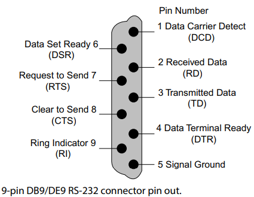
\includegraphics[width=.6\textwidth]{fig/fig3}
	\label{fig:fig3}
\end{figure}

\subsection{Dataoverførsel}
RS232 bruger asynkron dataoverførsel, hvilket betyder, at data sendes i et kontinuerligt strøm af bits uden en fast tidsbase. Dataoverførslen styres af start- og stopbits, som definerer begyndelsen og slutningen af hver dataramme. En typisk dataramme består af:
\begin{itemize}
	\item \textbf{Startbit}: 1 bit (logisk 0)
	\item \textbf{Databits}: 5 til 9 bits (typisk 8 bits)
	\item \textbf{Paritetsbit}: 1 bit (valgfri, bruges til fejlregistrering)
	\item \textbf{Stopbits}: 1, 1.5 eller 2 bits (logisk 1)
\end{itemize}

\subsection{Baudrate}
Baudrate refererer til antallet af signalændringer pr. sekund og bestemmer dataoverførselshastigheden. Typiske baudrater for RS232 er 9600, 19200, 38400, 57600 og 115200 baud. Det er vigtigt, at begge kommunikerende enheder er indstillet til samme baudrate for at sikre korrekt dataoverførsel.

\subsection{Fejlhåndtering}
RS232 anvender enkle fejlhåndteringsmetoder som paritetskontrol, hvor en ekstra bit føjes til hver dataramme for at gøre antallet af 1'er enten lige (even parity) eller ulige (odd parity). Hvis det modtagne antal 1'er ikke matcher den forventede paritet, registreres en fejl.

\subsection{Anvendelser}
RS232 er blevet brugt i en lang række applikationer, herunder:

\begin{itemize}
	\item Forbindelse af computere til modemmer
	\item Industriel automation og kontrolsystemer
	\item Seriel kommunikation med mikrokontrollere og indlejrede systemer
	\item Diagnostisk interface til netværksudstyr
\end{itemize}

\subsection{Fordele og Ulemper}
\begin{itemize}
	\item \textbf{Fordele:}
	\begin{itemize}
		\item Simpel og udbredt standard
		\item Velegnet til korte afstande og lave hastigheder
	\end{itemize}
	\item \textbf{Ulemper:}
	\begin{itemize}
		\item Begrænset dataoverførselshastighed og afstand
		\item Følsom overfor elektrisk støj
		\item Kræver flere ledninger til fuld duplex kommunikation
	\end{itemize}
\end{itemize}
RS232 har været en grundlæggende teknologi i mange år og bruges stadig i dag på trods af fremkomsten af mere avancerede serielle kommunikationsstandarder som USB og RS485.

\section{RS422}
RS422 (Recommended Standard 422) er en standard for seriel dataoverførsel, som er udviklet af Electronic Industries Alliance (EIA). RS422 blev designet til at forbedre de begrænsninger, der findes i RS232, især med hensyn til dataoverførselshastighed og afstand. RS422 anvender differentiel signalering, hvilket gør den mere robust overfor elektrisk støj og muliggør længere kommunikationsafstande.

\subsection{Fysiske Lag}
RS422 definerer det fysiske lag af kommunikationsforbindelsen, inklusive stiktyper, kabler og elektriske signaler. De mest almindelige stiktyper er DB9 (9-pins) og DB25 (25-pins), men andre konfigurationer findes også.
\begin{figure}[h]
	\centering
	
	\caption{DB9 stik for RS422}
	\label{fig:rs422_connector}
\end{figure}

\subsection{Elektriske Signaler}
RS422 bruger differentiel signalering, hvilket betyder, at signalet sendes som en spændingsforskel mellem to ledninger (A og B). Dette reducerer følsomheden overfor elektromagnetisk interferens (EMI). Typiske spændingsniveauer er:

\begin{itemize}
	\item \textbf{Logisk 0 (Marking)}: -2V til -6V (A-B)
	\item \textbf{Logisk 1 (Spacing)}: +2V til +6V (A-B)
\end{itemize}

\subsection{Signalering og Pins}
De vigtigste signaler og deres respektive pins i et DB9-stik er som følger:

\begin{itemize}
	\item \textbf{Pin 1}: GND (Signal Ground)
	\item \textbf{Pin 2}: TXD+ (Transmit Data Positive)
	\item \textbf{Pin 3}: TXD- (Transmit Data Negative)
	\item \textbf{Pin 4}: RXD+ (Receive Data Positive)
	\item \textbf{Pin 5}: RXD- (Receive Data Negative)
	\item \textbf{Pin 6-9}: Ikke brugt eller valgfri for kontrolsignaler
\end{itemize}

\subsection{Dataoverførsel}
RS422 understøtter asynkron og synkron dataoverførsel. Asynkron overførsel bruger start- og stopbits til at definere begyndelsen og slutningen af en dataramme, mens synkron overførsel bruger en klokkesignal til at synkronisere dataoverførslen.

\subsection{Baudrate og Afstand}
RS422 kan understøtte dataoverførselshastigheder op til 10 Mbps over korte afstande (op til 12 meter). Over længere afstande (op til 1200 meter) kan hastigheder op til 100 kbps opnås. Det er vigtigt at matche baudraten på begge kommunikerende enheder for at sikre korrekt dataoverførsel.

\subsection{Fejlhåndtering}
RS422's differentielle signalering reducerer fejl forårsaget af elektrisk støj. Desuden kan paritetskontrol og andre fejldetekteringsmetoder anvendes for at sikre dataintegritet.

\subsection{Anvendelser}
RS422 anvendes ofte i industrielle og kommercielle applikationer, herunder:
\begin{itemize}
	\item Industriel automation og kontrolsystemer
	\item Seriel kommunikation mellem computere og periferiudstyr
	\item Netværksforbindelser over lange afstande
	\item Kommunikationslinjer i høj EMI-miljøer
\end{itemize}

\subsection{Fordele og Ulemper}
\begin{itemize}
	\item \textbf{Fordele:}
	\begin{itemize}
		\item Højere dataoverførselshastigheder og længere rækkevidde sammenlignet med RS232.
		\item Robust overfor elektrisk støj på grund af differentiel signalering.
		\item Mulighed for at forbinde flere modtagere (op til 10) på samme sender.
	\end{itemize}
	\item \textbf{Ulemper:}
	\begin{itemize}
		\item Mere kompleks end RS232 med hensyn til kabelføring og stik.
		\item Kræver specielle drivere og modtagere til differentiel signalering.
	\end{itemize}
\end{itemize}
RS422 er en kraftfuld standard for seriel kommunikation, der tilbyder højere hastigheder og længere afstande end RS232, hvilket gør den velegnet til krævende industrielle applikationer.

\section{RS485}
RS485 (Recommended Standard 485) er en standard for seriel dataoverførsel, udviklet af Electronic Industries Alliance (EIA). RS485 er designet til at muliggøre pålidelig kommunikation over lange afstande og i støjfyldte miljøer. Den anvender differentiel signalering, som gør den robust overfor elektromagnetisk interferens (EMI) og tillader multi-drop netværk, hvor flere enheder kan kommunikere over samme bus.

\subsection{Fysiske Lag}
RS485 definerer det fysiske lag af kommunikationsforbindelsen, herunder stiktyper, kabler og elektriske signaler. De mest almindelige stiktyper er terminalblokke og DB9-stik.
\begin{figure}[h]
	\centering
	%\includegraphics[width=0.5\textwidth]{rs485_connector.png} % Inkluder et billede af RS485-stikket her
	\caption{Terminalblok stik for RS485}
	\label{fig:rs485_connector}
\end{figure}

\subsection{Elektriske Signaler}
RS485 bruger differentiel signalering, hvilket betyder, at signalet sendes som en spændingsforskel mellem to ledninger (A og B). Dette reducerer følsomheden overfor EMI. Typiske spændingsniveauer er:
\begin{itemize}
	\item \textbf{Logisk 0 (Marking)}: -1.5V til -5V (A-B)
	\item \textbf{Logisk 1 (Spacing)}: +1.5V til +5V (A-B)
\end{itemize}

\subsection{Signalering og Pins}
De vigtigste signaler og deres respektive pins i et typisk terminalblok-stik er som følger:
\begin{itemize}
	\item \textbf{Pin 1}: A (Data Line Positive)
	\item \textbf{Pin 2}: B (Data Line Negative)
	\item \textbf{Pin 3}: GND (Signal Ground)
	\item \textbf{Pin 4-5}: Valgfri for terminering eller skærmning
\end{itemize}

\subsection{Dataoverførsel}
RS485 understøtter både asynkron og synkron dataoverførsel. Asynkron overførsel bruger start- og stopbits til at definere begyndelsen og slutningen af en dataramme, mens synkron overførsel bruger et klokkesignal til at synkronisere dataoverførslen. RS485 tillader også multi-drop netværk, hvilket betyder, at op til 32 enheder kan tilsluttes på samme bus.

\subsection{Baudrate og Afstand}
RS485 kan understøtte dataoverførselshastigheder op til 10 Mbps over korte afstande (op til 15 meter). Over længere afstande (op til 1200 meter) kan hastigheder op til 100 kbps opnås. Det er vigtigt at matche baudraten på alle kommunikerende enheder for at sikre korrekt dataoverførsel.

\subsection{Fejlhåndtering}
RS485's differentielle signalering reducerer fejl forårsaget af elektrisk støj. Desuden kan paritetskontrol og andre fejldetekteringsmetoder anvendes for at sikre dataintegritet. RS485-netværk kan også bruge terminering modstande for at minimere refleksioner på kablet, hvilket forbedrer signalintegriteten.

\subsection{Anvendelser}
RS485 anvendes ofte i industrielle og kommercielle applikationer, herunder:
\begin{itemize}
	\item Industriel automation og kontrolsystemer
	\item Seriel kommunikation mellem computere og periferiudstyr
	\item Netværksforbindelser over lange afstande
	\item Kommunikationslinjer i høj EMI-miljøer
	\item Bygningsautomation (f.eks. HVAC-systemer, belysningskontrol)
\end{itemize}

\subsection{Fordele og Ulemper}
\begin{itemize}
	\item \textbf{Fordele:}
	\begin{itemize}
		\item Højere dataoverførselshastigheder og længere rækkevidde sammenlignet med RS232.
		\item Robust overfor elektrisk støj på grund af differentiel signalering.
		\item Mulighed for at forbinde op til 32 enheder på samme bus (kan udvides med repeaters).
	\end{itemize}
	\item \textbf{Ulemper:}
	\begin{itemize}
		\item Mere kompleks end RS232 med hensyn til kabelføring og stik.
		\item Kræver specielle drivere og modtagere til differentiel signalering.
		\item Kan være komplekst at konfigurere og fejlfinde i store netværk.
	\end{itemize}
\end{itemize}
RS485 er en kraftfuld standard for seriel kommunikation, der tilbyder højere hastigheder, længere afstande og multi-drop kapaciteter, hvilket gør den velegnet til krævende industrielle applikationer.

\section{DeviceNet}
DeviceNet er en industriel netværksprotokol, der bruges til at forbinde industrielle enheder såsom sensorer, aktuatorer og controllere. Det er en del af CIP (Common Industrial Protocol) og bruges ofte i automatiseringssystemer til at sikre pålidelig og effektiv kommunikation mellem enheder.

\subsection{Introduktion}
DeviceNet er designet til at være en fleksibel og skalerbar løsning til industriel kommunikation. Det giver mulighed for at tilføje og fjerne enheder uden at forstyrre det overordnede system, hvilket gør det ideelt til brug i dynamiske miljøer, hvor kravene til netværket kan ændre sig over tid.
\begin{figure}[!h]
	\centering
	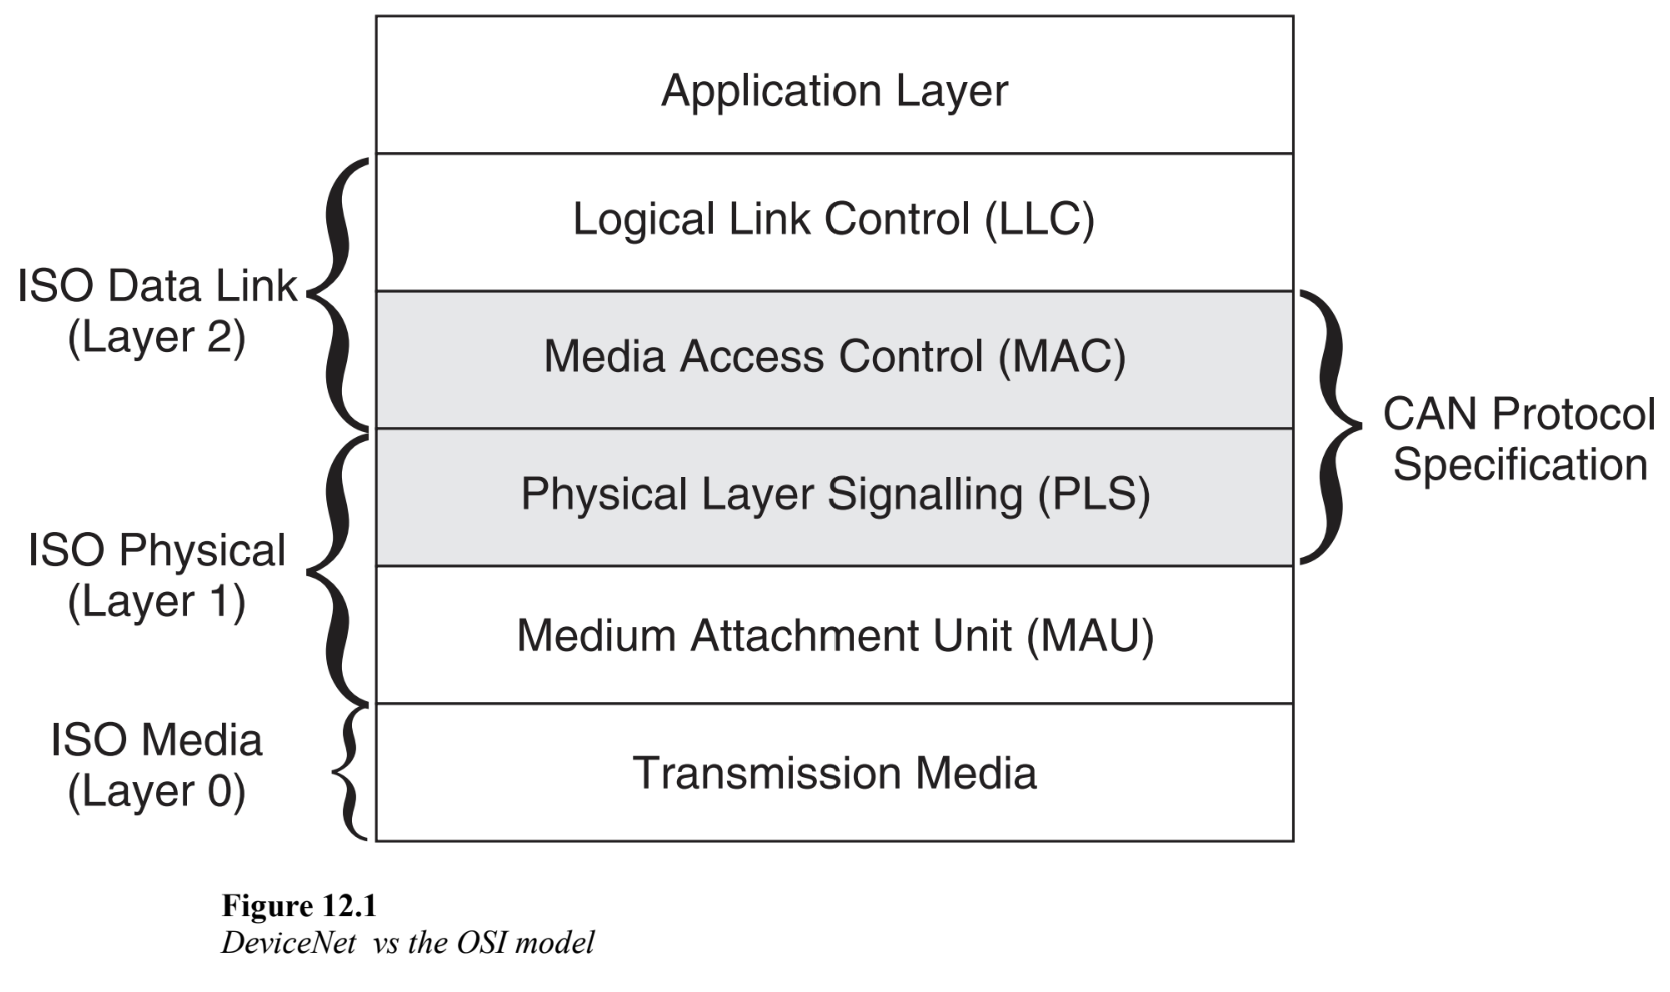
\includegraphics[width=\linewidth]{fig/fig13}
\end{figure}

\subsection{Fysisk Lag}
\subsection*{Topologi}
DeviceNet bruger en bus-topologi, hvor alle enheder er forbundet til en fælles kommunikationsbus. Dette layout er både simpelt og økonomisk, da det kræver minimal kabling og giver nem adgang til alle enheder på netværket. Det understøtter også stjerne- og trunk-line topologier, hvilket giver fleksibilitet i netværksdesign.

\subsection{Stikforbindelser}
\subsection*{Pluggbare (utætte) stik}
Disse stik er nemme at tilslutte og afbryde, hvilket gør dem ideelle til brug i miljøer, hvor hurtig installation og vedligeholdelse er nødvendig. De er dog ikke tætte og bør derfor ikke bruges i miljøer, hvor de kan udsættes for væsker eller støv.

\subsection*{Fastforbundne (utætte) stik}
Ligesom de pluggable stik er disse stik ikke tætte, men de giver en mere permanent forbindelse. De bruges ofte i mere stabile miljøer, hvor der ikke er behov for hyppig til- og frakobling.

\subsection*{Mini (tætte) stik}
Disse stik er designet til at være tætte og beskytte mod indtrængen af væsker og støv. De er ideelle til brug i barske industrielle miljøer.

\subsection*{Mikro (tætte) stik}
Mikrostik er mindre end mini-stik, men tilbyder samme niveau af tæthed. De bruges ofte i applikationer, hvor pladsen er begrænset.

\subsection{Kabelbudgetter}
Kabelbudgetter i DeviceNet bestemmer den maksimale længde og type af kabel, der kan bruges, uden at det påvirker netværkets ydeevne. Dette inkluderer overvejelser om signalstyrke, spændingsfald og dataoverførselshastigheder.

\subsection{Enhedstaps}
\subsection*{Tætte taps}
Tætte taps giver en sikker forbindelse, der beskytter mod indtrængen af væsker og støv. De bruges i miljøer, hvor pålidelighed og beskyttelse er afgørende.

\subsection*{IDC taps}
IDC (Insulation Displacement Connector) taps er nemme at installere og kræver ikke, at kablets isolering fjernes. Dette gør installationen hurtigere og reducerer risikoen for skader på kablet.

\subsection*{Åbne taps}
Åbne taps er ikke beskyttede mod miljøpåvirkninger og bør kun bruges i kontrollerede indendørs miljøer.

\subsection*{Multiport åbne taps}
Disse taps giver mulighed for tilslutning af flere enheder på samme punkt, hvilket kan reducere kablingsomkostningerne og forenkle installationen.

\subsection*{Strømtaps}
Strømtaps giver en dedikeret forbindelse til strømforsyning af enheder på netværket, hvilket kan være nødvendigt i applikationer med høje strømkrav.

\subsection{Kabler}
\subsection*{Tykt kabel}
Tykt kabel bruges i DeviceNet-applikationer, hvor lange kabellængder eller høje strømkrav er nødvendige. Det giver lavere modstand og bedre signalintegritet over lange afstande.

\subsection*{Tyndt kabel}
Tyndt kabel bruges i applikationer, hvor pladsen er begrænset, og kabellængderne er korte. Det er lettere at håndtere og installere i trange rum.

\subsection*{Fladt kabel}
Fladt kabel bruges i applikationer, hvor kablet skal lægges under gulve eller tæpper. Det er nemt at skjule og giver en pænere installation.

\subsection{Netværksstrøm}
\subsection*{Generel tilgang}
Netværksstrøm i DeviceNet sikrer, at alle enheder på netværket får tilstrækkelig strøm til at fungere korrekt. Dette inkluderer overvejelser om strømforsyningens kapacitet og distribution.

\subsection*{Enkel forsyning – ende tilsluttet}
Denne tilgang til netværksstrøm bruger en enkelt strømforsyning, der er tilsluttet i enden af netværket. Dette er en simpel og økonomisk løsning, men kan være mindre pålidelig i store netværk.

\subsection*{Enkel forsyning – midter tilsluttet}
Denne tilgang placerer strømforsyningen i midten af netværket, hvilket giver en mere jævn fordeling af strømmen og kan forbedre pålideligheden i større netværk.

\subsection*{Forslag til undgåelse af fejl og strømforsyningsmuligheder}
For at undgå fejl i netværksstrømmen skal der tages højde for faktorer som korrekt dimensionering af strømforsyningen, brug af redundante strømforsyninger og regelmæssig vedligeholdelse.

\subsection{Systemjord}
Systemjord sikrer, at alle enheder på netværket har en fælles jordforbindelse, hvilket er afgørende for at undgå jordsløjfer og signalstøj.

\subsection{Signalering}
DeviceNet bruger signaleringsteknikker til at kommunikere data mellem enheder. Dette inkluderer brugen af specifikke spændingsniveauer og tidsrammer for at sikre pålidelig dataoverførsel.

\subsection{Data Link Lag}	
\subsection*{Rammeformat}
Rammeformatet i DeviceNet definerer strukturen af de data, der overføres mellem enheder. Dette inkluderer felter som start- og stopbits, adresseinformation og fejlkontrol.

\subsection*{Mediumadgang}
Mediumadgang kontrollerer, hvordan enheder får adgang til kommunikationsmediet. DeviceNet bruger en deterministisk tilgang, hvor hver enhed tildeles et bestemt tidspunkt til at sende data.

\subsection*{Fragmentering}
Fragmentering bruges til at opdele store datarammer i mindre dele, der kan overføres effektivt over netværket. Disse fragmenter samles igen ved modtageren for at gendanne den oprindelige data.

\subsection{Applikationslaget}
Applikationslaget i DeviceNet definerer de protokoller og services, der bruges til at udføre specifikke funktioner, såsom læsning og skrivning af data, alarmhåndtering og diagnostik.

\subsection{Fejlfinding}
\subsection*{Introduktion}
Fejlfinding i DeviceNet involverer identifikation og løsning af problemer, der kan påvirke netværkets ydeevne og pålidelighed.

\subsection*{Værktøjer til fejlfinding}
Værktøjer som netværksscannere, multimetre og protokolanalysatorer kan bruges til at diagnosticere problemer i DeviceNet-netværk.

\subsection*{Fejlfindingsprocedurer}
Fejlfindingsprocedurer inkluderer systematisk kontrol af kabler, stik, strømforsyninger og netværkskonfigurationer for at identificere og løse problemer.
\clearpage
\subsection{Opsummering}
DeviceNet er en robust og fleksibel netværksprotokol, der er designet til at opfylde kravene i moderne industrielle automatiseringssystemer. Ved at forstå de forskellige aspekter af DeviceNet, fra fysisk lag til applikationslag og fejlfinding, kan teknikere og ingeniører sikre, at deres netværk fungerer optimalt og pålideligt.
\begin{figure}[!h]
	\centering
	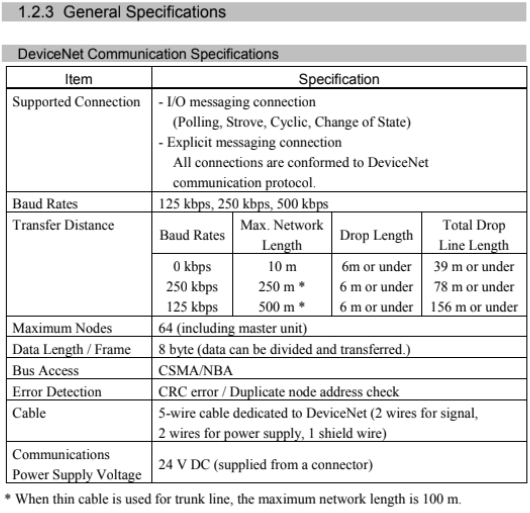
\includegraphics[width=.8\linewidth]{fig/fig14}
\end{figure}
\clearpage
\section{ProfiBus PA/DP/FMS Overview}
ProfiBus (Process Field Bus) er en standardiseret industrielt kommunikationsprotokol, der bruges til at forbinde automatiseringsenheder som sensorer, aktuatorer og controllere. Det er en af de mest udbredte feltbusstandarder i verden og understøtter både procesautomatisering (PA), decentraliseret periferikommunikation (DP) og feltbussystemer (FMS).

\subsection{Introduktion}
ProfiBus er udviklet til at muliggøre hurtig og pålidelig kommunikation mellem industrielle enheder. Det er en alsidig protokol, der kan bruges i en bred vifte af applikationer, herunder fabriksautomatisering, proceskontrol og bygningsautomatisering.

\subsection{ProfiBus Protocol Stack}
ProfiBus-protokollen er opdelt i flere lag, som hver især håndterer forskellige aspekter af kommunikationen. Denne lagdelte arkitektur gør det muligt at isolere og håndtere forskellige funktioner effektivt.

\subsection*{Fysisk Lag (Layer 1)}
Det fysiske lag i ProfiBus definerer de elektriske og mekaniske egenskaber ved netværksforbindelserne. Dette inkluderer specifikationer for kabler, stik og elektriske signaler, der bruges til at overføre data mellem enheder.

\subsection*{Datalink Lag (Layer 2)}
Datalink-laget håndterer pålidelig overførsel af data mellem enheder på netværket. Dette inkluderer fejlregistrering og korrektion, adressering af enheder og styring af datarammer.

\subsection*{Applikationslag}
Applikationslaget definerer de protokoller og tjenester, der bruges til at udføre specifikke funktioner som læsning og skrivning af data, alarmhåndtering og diagnostik. Dette lag sikrer, at applikationer kan kommunikere effektivt over netværket.

\subsection*{Fieldbus Message Specification (FMS)}
FMS specificerer de meddelelser, der bruges til at kommunikere mellem enheder på feltbusnetværket. Dette inkluderer standarder for meddelelsesformat og kommunikationsprotokoller.

\subsection*{Lower Layer Interface (LLI)}
LLI fungerer som en grænseflade mellem de lavere lag (fysisk og datalink) og de højere lag (applikation og FMS). Det sikrer, at data kan overføres effektivt mellem disse lag.

\subsection*{Fieldbus Management Layer (FMA 7)}
FMA 7 håndterer styring og konfiguration af feltbusnetværket. Dette inkluderer opgaver som netværksinitialisering, konfigurationsstyring og diagnosticering af netværksfejl.

\subsection{ProfiBus Kommunikation Model}
ProfiBus kommunikationsmodellen beskriver, hvordan data overføres mellem enheder på netværket. Dette inkluderer beskrivelser af kommunikationscyklusser, dataoverførselshastigheder og synkroniseringsmetoder.

\subsection{Forhold mellem Applikationsproces og Kommunikation}
Dette afsnit beskriver, hvordan applikationsprocesser interagerer med kommunikationsprotokollen for at sikre effektiv dataoverførsel. Det forklarer, hvordan data fra applikationslaget omsættes til meddelelser, der kan sendes over netværket.

\subsection{Kommunikationsobjekter}
Kommunikationsobjekter i ProfiBus refererer til de enheder, data og tjenester, der kan adresseres og styres over netværket. Dette inkluderer beskrivelser af de forskellige typer af kommunikationsobjekter og deres funktioner.

\subsection{Ydeevne}
Dette afsnit diskuterer ydeevnen af ProfiBus-netværket, herunder dataoverførselshastigheder, responstider og netværkskapacitet. Det giver også retningslinjer for optimering af netværksydeevne.

\subsection{Systemoperation}
\subsection*{Konfiguration}
ProfiBus-netværket kræver korrekt konfiguration for at fungere optimalt. Dette afsnit beskriver de trin, der er nødvendige for at konfigurere enheder, tildele adresser og indstille netværksparametre.

\subsection*{Dataoverførsel mellem DPM1 og DP-slaver}
Dette afsnit beskriver processen for dataoverførsel mellem masterenheden (DPM1) og slaveenhederne (DP-slaver). Det forklarer, hvordan data pakkes, adresseres og sendes over netværket.

\subsection*{Synkronisering og Frysemodi}
Synkronisering og frysemodi bruges til at koordinere dataoverførsel mellem enheder og sikre, at dataene overføres på det rigtige tidspunkt. Dette afsnit beskriver, hvordan disse funktioner implementeres og bruges.

\subsection*{Sikkerhed og Beskyttelse af Stationer}
Sikkerhed og beskyttelse er afgørende for at sikre, at netværket fungerer pålideligt og uden forstyrrelser. Dette afsnit beskriver de mekanismer, der bruges til at beskytte netværket mod fejl og angreb.

\subsection*{Blandet Drift af FMS- og DP-stationer}
Dette afsnit beskriver, hvordan FMS- og DP-stationer kan fungere samtidigt på samme netværk. Det forklarer, hvordan kompatibilitet og interoperabilitet sikres mellem forskellige typer enheder.

\subsection{Fejlfinding}
\subsection*{Introduktion}
Fejlfinding er en vigtig del af vedligeholdelsen af ProfiBus-netværket. Dette afsnit introducerer de grundlæggende principper for fejlfinding og diagnosticering af netværksproblemer.

\subsection*{Fejlfinding Værktøjer}
Der findes forskellige værktøjer, der kan bruges til at diagnosticere og løse problemer i ProfiBus-netværket. Dette afsnit beskriver nogle af de mest almindelige værktøjer og deres anvendelser.

\subsection*{Tips}
Dette afsnit giver praktiske tips til fejlfinding og vedligeholdelse af ProfiBus-netværket. Det inkluderer anbefalinger til forebyggelse af almindelige problemer og optimering af netværksydelsen.

\subsection{Opsummering}
ProfiBus er en alsidig og pålidelig feltbusprotokol, der er designet til at opfylde behovene i moderne industrielle automatiseringssystemer. Ved at forstå de forskellige aspekter af ProfiBus, fra protokolstack til fejlfinding, kan teknikere og ingeniører sikre, at deres netværk fungerer effektivt og pålideligt.
\begin{figure}[!h]
	\centering
	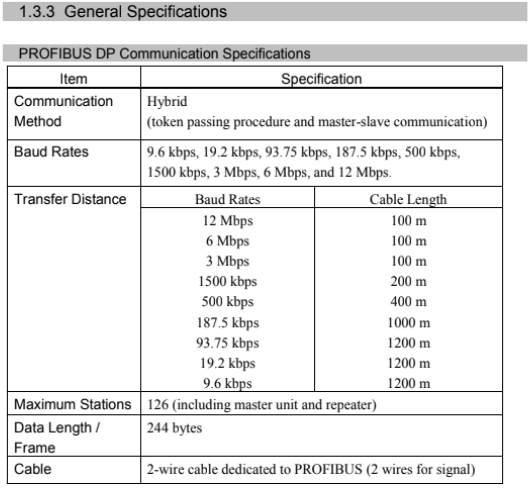
\includegraphics[width=\linewidth]{fig/fig15}
\end{figure}
